\documentclass[10pt]{article}
\usepackage{tikz}
\usetikzlibrary{shapes.misc}
\usepackage[margin=0cm]{geometry}
\pagestyle{empty}
\tikzstyle{every node}=[cross out, draw, red]

\begin{document}

\vspace*{\fill}
\begin{center}
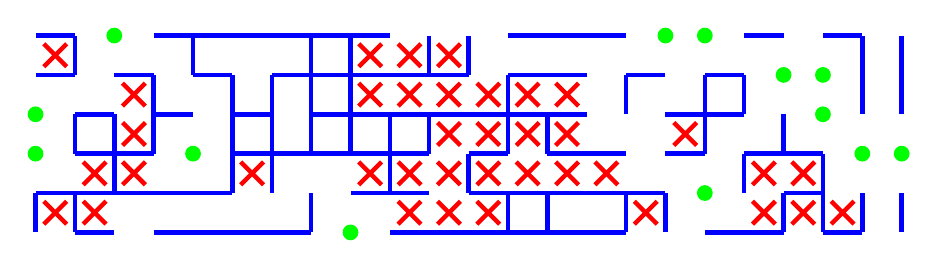
\begin{tikzpicture}[x=0.5cm, y=-0.5cm, ultra thick, blue]
% Walls
    \draw (0,0) -- (1,0);
    \draw (3,0) -- (9,0);
    \draw (12,0) -- (15,0);
    \draw (18,0) -- (19,0);
    \draw (20,0) -- (21,0);
    \draw (0,1) -- (1,1);
    \draw (2,1) -- (3,1);
    \draw (4,1) -- (5,1);
    \draw (6,1) -- (11,1);
    \draw (12,1) -- (14,1);
    \draw (15,1) -- (16,1);
    \draw (17,1) -- (18,1);
    \draw (1,2) -- (2,2);
    \draw (3,2) -- (4,2);
    \draw (5,2) -- (6,2);
    \draw (7,2) -- (14,2);
    \draw (16,2) -- (18,2);
    \draw (1,3) -- (3,3);
    \draw (5,3) -- (10,3);
    \draw (11,3) -- (12,3);
    \draw (13,3) -- (15,3);
    \draw (16,3) -- (17,3);
    \draw (18,3) -- (20,3);
    \draw (0,4) -- (5,4);
    \draw (8,4) -- (10,4);
    \draw (11,4) -- (16,4);
    \draw (19,4) -- (20,4);
    \draw (1,5) -- (2,5);
    \draw (3,5) -- (7,5);
    \draw (9,5) -- (15,5);
    \draw (17,5) -- (19,5);
    \draw (20,5) -- (21,5);
    \draw (0,4) -- (0,5);
    \draw (1,0) -- (1,1);
    \draw (1,2) -- (1,3);
    \draw (1,4) -- (1,5);
    \draw (2,2) -- (2,4);
    \draw (3,1) -- (3,3);
    \draw (4,0) -- (4,1);
    \draw (5,1) -- (5,4);
    \draw (6,1) -- (6,4);
    \draw (7,0) -- (7,3);
    \draw (7,4) -- (7,5);
    \draw (8,0) -- (8,3);
    \draw (9,2) -- (9,4);
    \draw (10,0) -- (10,1);
    \draw (10,2) -- (10,3);
    \draw (11,0) -- (11,1);
    \draw (11,3) -- (11,4);
    \draw (12,1) -- (12,3);
    \draw (12,4) -- (12,5);
    \draw (13,2) -- (13,3);
    \draw (13,4) -- (13,5);
    \draw (15,1) -- (15,2);
    \draw (15,4) -- (15,5);
    \draw (16,4) -- (16,5);
    \draw (17,1) -- (17,3);
    \draw (18,1) -- (18,2);
    \draw (18,3) -- (18,4);
    \draw (19,2) -- (19,3);
    \draw (19,4) -- (19,5);
    \draw (20,3) -- (20,5);
    \draw (21,0) -- (21,2);
    \draw (21,4) -- (21,5);
    \draw (22,0) -- (22,2);
    \draw (22,4) -- (22,5);
% Pillars
    \fill[green] (2,0) circle(0.2);
    \fill[green] (16,0) circle(0.2);
    \fill[green] (17,0) circle(0.2);
    \fill[green] (19,1) circle(0.2);
    \fill[green] (20,1) circle(0.2);
    \fill[green] (0,2) circle(0.2);
    \fill[green] (20,2) circle(0.2);
    \fill[green] (0,3) circle(0.2);
    \fill[green] (4,3) circle(0.2);
    \fill[green] (21,3) circle(0.2);
    \fill[green] (22,3) circle(0.2);
    \fill[green] (17,4) circle(0.2);
    \fill[green] (8,5) circle(0.2);
% Inner points in accessible cul-de-sacs
    \node at (0.5,0.5) {};
    \node at (8.5,0.5) {};
    \node at (9.5,0.5) {};
    \node at (10.5,0.5) {};
    \node at (2.5,1.5) {};
    \node at (8.5,1.5) {};
    \node at (9.5,1.5) {};
    \node at (10.5,1.5) {};
    \node at (11.5,1.5) {};
    \node at (12.5,1.5) {};
    \node at (13.5,1.5) {};
    \node at (2.5,2.5) {};
    \node at (10.5,2.5) {};
    \node at (11.5,2.5) {};
    \node at (12.5,2.5) {};
    \node at (13.5,2.5) {};
    \node at (16.5,2.5) {};
    \node at (1.5,3.5) {};
    \node at (2.5,3.5) {};
    \node at (5.5,3.5) {};
    \node at (8.5,3.5) {};
    \node at (9.5,3.5) {};
    \node at (10.5,3.5) {};
    \node at (11.5,3.5) {};
    \node at (12.5,3.5) {};
    \node at (13.5,3.5) {};
    \node at (14.5,3.5) {};
    \node at (18.5,3.5) {};
    \node at (19.5,3.5) {};
    \node at (0.5,4.5) {};
    \node at (1.5,4.5) {};
    \node at (9.5,4.5) {};
    \node at (10.5,4.5) {};
    \node at (11.5,4.5) {};
    \node at (15.5,4.5) {};
    \node at (18.5,4.5) {};
    \node at (19.5,4.5) {};
    \node at (20.5,4.5) {};
% Entry-exit paths without intersections
\end{tikzpicture}
\end{center}
\vspace*{\fill}

\end{document}
